% !TEX TS-program = pdflatex
% Source of Graphics/PlotBad.pdf, the badly drawn plot in Chapter 4 of the
% sample. It is made with pgfplots; compile it on its own with pdflatex.
% Its faults are deliberate: hairline curves, a tiny legend over the data,
% Helvetica labels that do not match the Times text, curves told apart
% only by red and pure green (RGB [0 1 0], nearly invisible on white),
% cryptic axis labels without units, and a heavy
% grid. A red cross is drawn over the whole plot.
\documentclass[border=2pt]{standalone}
\usepackage[scaled]{helvet}
\renewcommand{\familydefault}{\sfdefault}
\usepackage{pgfplots}
\pgfplotsset{compat=1.16}
\begin{document}
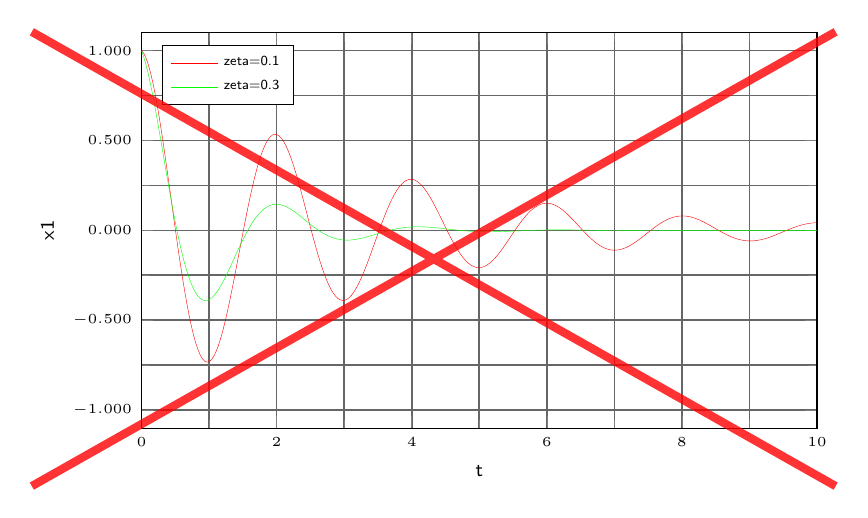
\begin{tikzpicture}
\begin{axis}[
  width=4in, height=2.6in,
  xlabel={t}, ylabel={x1},
  xmin=0, xmax=10, ymin=-1.1, ymax=1.1,
  grid=both, grid style={black!60, line width=0.6pt},
  minor tick num=1,
  tick label style={font=\tiny},
  label style={font=\scriptsize},
  y tick label style={/pgf/number format/.cd, fixed, fixed zerofill, precision=3},
  legend style={font=\fontsize{4}{5}\selectfont, at={(0.03,0.97)}, anchor=north west},
]
\addplot[red, line width=0.15pt, samples=300, domain=0:10]
  {exp(-0.1*2*pi*0.5*x)*cos(deg(2*pi*0.5*sqrt(1-0.01)*x))};
\addplot[color={rgb,1:red,0;green,1;blue,0}, line width=0.15pt, samples=300, domain=0:10]
  {exp(-0.3*2*pi*0.5*x)*cos(deg(2*pi*0.5*sqrt(1-0.09)*x))};
\legend{zeta=0.1, zeta=0.3}
\end{axis}
% The red cross over the whole plot
\draw[red, line width=3pt, opacity=0.8]
  (current bounding box.south west) -- (current bounding box.north east)
  (current bounding box.north west) -- (current bounding box.south east);
\end{tikzpicture}
\end{document}
